\section{Minimal number of measurements with random matrices}

From now on we will consider only random matrices with $\mathcal{N}(0,1)$-distributed entries.
It might seem unnatural at first if we think of compressive sensing only in the context of natural phenomena, where we have no
or little control over how vector $\y$ is obtained.
However, we could also look, for example, at data compression, where we are free to choose the matrix $\A$ however we like.
Considering the vast number of results for normally distributed matrices and normal distribution in general,
they become convenient candidates for the task.

Before proceeding to the recovery conditions for random matrices, we first have to recall some definitions from convex geometry,
relying mainly on \cite{rockafellar} as source material.

\begin{definition}
    A convex set $\mathcal{C} \subset \mathbb{R}^N$ is called a \textit{cone} if it is closed under non-negative scalar multiplications, i.e.
    $\forall \alpha \geq 0, \x \in \mathcal{C}: \alpha \x \in \mathcal{C}$.

    The cone $\mathcal{C}^* = \{ \x \in \mathbb{R}^N : \left< \x, \y \right> \leq 0, \ \forall \y \in \mathcal{C} \}$
    is called the \textit{polar} of $\mathcal{C}$.
\end{definition}

\begin{definition}
    Let $C \subset \mathbb{R}^N$ be a convex set and $\x \in \mathbb{R}^N$.
    We call a \textit{tangent cone} of $C$ the cone $T_C(\x) = \op{cl}\{\alpha\x: \x \in C, \alpha \geq 0  \} $.
    We call a \textit{normal cone} of $C$ the cone $N_C(\x) = T_C^*(\x)$.
\end{definition}

\begin{definition}
    The \textit{descent cone} $\mathcal{D}(f, \x) $ of a proper convex function $f: \mathbb{R}^N \rightarrow \overline{\mathbb{R}}$
    at $\x \in \mathbb{R}^N$ is defined as $$\mathcal{D}(f, \x) = \bigcup_{\tau > 0} \left\{ \z \in \mathbb{R}^N: f(\x+\tau \z) \leq f(\x) \right\}. $$
\end{definition}

\begin{remark}
    Descent cones are closely related to sublevel sets; in fact, $T_C(\x) = \op{cl} \mathcal{D}(f, \x)$
    for $C = \{\z: f(\z) \leq f(\x)\}$.
    In \cite{convexgeom}, authors formulate the following result with tangent cones to sublevel sets instead.
    However, we will use descent cones as is done in \cite{lote}.
\end{remark}

\begin{figure}
    \begin{subfigure}{0.45\textwidth}
        \begin{tikzpicture}
            \path [fill=teal, fill opacity=0.15] (0, 2) -- (-3.5, -1.5) to[curve through={(-2.5, -2.6) .. (-1.8, -2.7) .. (0, -3.4) ..
            (1.3, -2.9) .. (2, -2.8)}] (3.5, -1.5) -- (0, 2) --cycle;
            \draw [gray, densely dashed][->] (-3.5,0)--(3.5,0);
            \draw [gray, densely dashed][->] (0,-2.2)--(0,3);
            \draw [gray, densely dashed] (0, -3.5) -- (0, -2.8)
            \draw [teal, draw opacity=0.5] (0, 2) -- (-3.5, -1.5);
            \draw [teal, draw opacity=0.5] (0, 2) -- (3.5, -1.5);
            \draw [teal, line width=1pt][shorten <=-3cm] (0,2)--(3.5, 1) node [sloped, pos=0.7, above=-0.1cm] {$\op{Ker}\A+\x^*$};
            \draw [pattern=vertical lines, fill opacity=0.25](-2,0)--(0,2)--(2,0)--(0,-2)--cycle;
            \draw[black] [-{Circle[width=3pt, length=3pt, fill=black, black]}, shorten >=-1.5pt] (0,2) node [above right] {$\x^*$};
            \node at (0, -2.5) {$\mathcal{D}(\norm{\cdot}_1, \x^*)+\x^*$};
        \end{tikzpicture}
        \caption{}
    \end{subfigure}
    \hfill
    \begin{subfigure}{0.45\textwidth}
        \begin{tikzpicture}
            \path [fill=teal, fill opacity=0.15] (0, 2) -- (-3.5, -1.5) to[curve through={(-2.5, -2.6) .. (-1.8, -2.7) .. (0, -3.4) ..
            (1.3, -2.9) .. (2, -2.8)}] (3.5, -1.5) -- (0, 2) --cycle;
            \draw [gray, densely dashed][->] (-3.5,0)--(3.5,0);
            \draw [gray, densely dashed][->] (0,-2.2)--(0,3);
            \draw [gray, densely dashed] (0, -3.5) -- (0, -2.8)
            \draw [teal, draw opacity=0.5] (0, 2) -- (-3.5, -1.5);
            \draw [teal, draw opacity=0.5] (0, 2) -- (3.5, -1.5);
            \draw [teal, line width=1pt][shorten <=-1cm] (0,2)--(2.5, -3.5) node [pos=0, above left=0.3cm] {$\op{Ker}\A+\x^*$};
            \draw [pattern=vertical lines, fill opacity=0.25](-2,0)--(0,2)--(2,0)--(0,-2)--cycle;
            \draw[black] [-{Circle[width=3pt, length=3pt, fill=black, black]}, shorten >=-1.5pt] (0,2) node [above right] {$\x^*$};
            \node at (0, -2.5) {$\mathcal{D}(\norm{\cdot}_1, \x^*)+\x^*$};
        \end{tikzpicture}
        \caption{}
    \end{subfigure}
    \caption{\centering Colored area shows the descent cone to the $l_1$ norm in $\x^*$; dashed area is the set of vectors for which
    the norm is decreasing compared to $\x^*$.}
    \label{fig:desc_cone}
\end{figure}

\begin{proposition}
    The vector $\x \in \mathbb{R}^N$ is the unique solution of \ref{eq:l1} with $\y = \A\x$ if and only if
    $\mathcal{D}(\norm{\cdot}_1, \x) \cap \op{Ker} \A = \{\mathbf{0}\}$.
    \label{th:ker}
\end{proposition}

\begin{proof}
    $(\Leftarrow)$ Let $\x \in \mathbb{R}^N$ and $\mathcal{D}(\norm{\cdot}_1, \x) \cap \op{Ker} \A = \{\mathbf{0}\}$.
    Additionally, we assume that vector $\x$ satisfies linear constraints $\A\x=\y$.
    Suppose that there exists $\z \in \mathbb{R}^N$, $\z \neq \x$, such that $\A\z=\y$ and $\norm{z}_1 \leq \norm{x}_1$.
    Then $\A(\z-\x)=0$ and $z-x \in \op{Ker} \A$.
    By definition, $\mathcal{D}(f, \x) = \bigcup_{\tau > 0} \left\{ \z \in \mathbb{R}^N: \norm{\x+\tau \z}_1 \leq \norm{\x} \right\}$.
    So, $\z - \x \in \mathcal{D}(\norm{\cdot}_1, \x)$ (with $\tau = 1$ we have $\norm{\x + (\z - \x)}_1 \leq \norm{\x}_1$).
    But then $\mathcal{D}(\norm{\cdot}_1, \x) \cap \op{Ker} \A \neq \{\mathbf{0}\}$, which contradicts the hypothesis.
    Thus, $\x$ is the unique minimizer of~\ref{eq:l1}.

    $(\Rightarrow)$ Let $\x \in \mathbb{R}^N$ be the unique solution of~\ref{eq:l1}, i.e, $\x$ satisfies $\A\x=\y$ and
    for any $\x' \neq \x$ such that $\A \x' = \y$, $\norm{\x'}_1 > \norm{\x}_1$.
    Let $\z \in \mathcal{D}(\norm{\cdot}_1, \x)$ and $\z \neq \mathbf{0}$.
    Then there exists $\tau > 0$ such that $\norm{\x + \tau \z}_1 \leq \norm{\x}_1 $.
    If we suppose that $\z \in \op{Ker} \A$, then $\A \z = \mathbf{0}$ and $\A(\x + \tau \z) = \y$.
    As $\x$ is the unique minimizer, it has to be that $\norm{\x + \tau \z}_1 > \norm{\x}_1$, which leads to a contradiction.
    Thus, $\mathcal{D}(\norm{\cdot}_1, \x) \cap \op{Ker} \A = \{\mathbf{0}\}$.
\end{proof}

The visual interpretation of this result can be seen in Fig~\ref{fig:desc_cone}.
If kernel intersects the descent cone in more than just $\mathbf{0}$, then there exists $\z \in \op{Ker}\A$ such that
$\norm{\z+\x^*}_1 \leq \norm{\x^*}_1$.
Also, $\A (\z+\x^*) = \y$ and thus $\x^*$ is not the unique solution of \ref{eq:l1}.

Now that we have the foundation laid down, let us move onto the main part of this report.
Most of the time during the project was spent on working with two papers: ``The Convex Geometry of Linear Inverse Problems''
by V.~Chandrasekaran et al. (2012) and ``Living on the edge: Phase transitions in convex programs with random data''
by D.~Amelunxen et al. (2013).
Those papers take Proposition~\ref{th:ker} and ask a question: what is the probability of the descent cone and the kernel
to intersect (other than in $\mathbf{0}$)?
To answer that question they propose two different ways to ``measure'' how big the cone is compared to the ambient
dimension.
The second paper goes further than that and also studies the phase transition that happens as we increase $m$.
We will discuss the minimal theory behind those two papers and look at some numerical experiments in the following sections.

\subsection{The Convex Geometry of Linear Inverse Problems}

Authors of this paper didn't limit their study to $l_1$-minimization; they also study adjacent sparsity-related problems
by introducing \textit{atomic norms}.
However, we are not interested in generality right now, so we will formulate all the results in restriction to $l_1$ norm.
Conveniently enough, it also makes connections with the next paper more apparent, as we can utilise descent cones here as well.
The only thing left to define is Gaussian width.

\begin{figure}
    \begin{subfigure}{0.5\linewidth}
        \includegraphics[width=\linewidth]{pictures/log_estimate.png}
        \caption{}
    \end{subfigure}
    \begin{subfigure}{0.5\linewidth}
        \includegraphics[width=\linewidth]{pictures/log_estimate300.png}
        \caption{}
    \end{subfigure}
    \caption{\centering Results of numerical experiments in dimensions 100 and 300. The red line represents the minimal $m$ required by
    Corollary~\ref{th:log}.}
    \label{fig:log}
\end{figure}

%\begin{definition}
%    Let $\mathcal{A} \subset \mathbb{R}^{N}$ be a compact set of atoms.
%    The atomic norm of $\x \in \mathbb{R}^N$ is then defined as
%    \[ \norm{\x}_\mathcal{A} = \inf \left\{  \sum_{\mathbf{a} \in \mathcal{A}}c_\mathbf{a}:
%                                        \x = \sum_{\mathbf{a} \in \mathcal{A}}c_\mathbf{a} \mathbf{a},
%        ~c_\mathbf{a} \geq 0 \ \forall\mathbf{a} \in \mathcal{A} \right\}. \]
%\end{definition}
%
%We will be interested only in the specific case of the $l_1$ norm which can be interpreted as an atomic norm with
%$\mathcal{A} = \cup_{k=1}^N \{ \mathbf{e}^{(k)}: e^{(k)}_k = 1, e^{(k)}_j = 0 \ \forall j \neq k \}$, i.e., the standard basis.

\begin{definition}
    The \textit{Gaussian width} of a set $S \subset \mathbb{R}^N$ is defined as
    \[ w(S) = \mathbb{E} \left[ \sup_{\z \in S} \mathbf{g}^T \z \right], \]
    where $\mathbf{g} \sim \mathcal{N}(\mathbf{0}, \mathbf{I})$ is a vector of i.i.d. random variables with standard normal distribution.
\end{definition}

The following two results are the most important ones for us; they tell us when we can recover vector $\x^*$ from \ref{eq:l1}.

\begin{theorem}\label{th:yibucha}
    Let $\A \in M_{m \times N}$ be a random matrix with i.i.d components with $\mathcal{N}(0, 1)$ distribution,
    $\x^* \in \mathbb{R}^N$ and let $\Omega = \mathcal{D}(\norm{\cdot}_1, \x^*) \cap \mathbb{S}^{N-1}$.
    Suppose that $\y = \A \x^*$.
    Then
    \[ m \geq w(\Omega)^2 + 1 \implies \mathbb{P}\{ \x^* \text{ is the unique solution of \ref{eq:l1}} \} \geq
    1-\exp\left(-\frac{1}{2}(\lambda_m - w(\Omega))^2\right),\]
    where $\lambda_m$ is the expected length of an $m$-dimensional gaussian vector.
\end{theorem}

\begin{proposition}
    Let $\x^* \in \mathbb{R}^N$ be an $s$-sparse vector.
    We have the following inequality:
    \[ w(\mathcal{D}(\norm{\cdot}_1, \x^*)\cap \mathbb{S}^{N-1})^2 \leq 2s \log \frac{N}{s} + \frac{5}{4}s.\]
\end{proposition}
If we combine this result with Theorem~\ref{th:yibucha}, we get the following condition for successful recovery:
\begin{corollary}\label{th:log}
    Let $\x^* \in \mathbb{R}^N$ be an $s$-sparse vector with $\y = \A \x^*$.
    Then $2s\log \frac{N}{s} + \frac{5}{4}s + 1$ measurements suffice to recover $\x^*$ from \ref{eq:l1} with high probability, i.e.,
    \begin{multline}
        m \geq 2s\log \frac{N}{s} + \frac{5}{4}s + 1 \implies \\
        \mathbb{P}\{\x^* \text{ is the unique solution of \ref{eq:l1}}\} \geq
        1 - \exp \left( - \frac{1}{2} \left[\lambda_m - w(\Omega)\right]^2 \right).
        \label{eq:log}
    \end{multline}
\end{corollary}
In Fig.~\ref{fig:log} we can see this estimate applied to dimensions 100 and 300.

\begin{figure}
    \begin{subfigure}{0.5\textwidth}
        \includegraphics[width=\linewidth]{pictures/log_proba100}
        \caption{}
    \end{subfigure}
    \begin{subfigure}{0.5\textwidth}
        \includegraphics[width=\linewidth]{pictures/log_proba1000}
        \caption{}
    \end{subfigure}
    \caption{\centering Plots for the probability estimate as seen in (\ref{eq:log_improved}).
    In (a) $N=100$, $s=10$, while in (b) $N=1000$, $s=100$.}
    \label{fig:log-proba}
\end{figure}

\begin{remark}
    In the paper, authors formulate this result without specifying the probability and just referring to it as being ``high''.
    And it is, no doubt, high; however, we can try studying that in more detail.
    At this point, the expression for probability contains $w(\Omega)$, which is not great for numerical experiments.
    The next lemma gives a probability estimate that depends explicitly on $m$, $s$ and $N$.
\end{remark}

\begin{lemma} \label{th:log_improved}
    Let $\x^* \in \mathbb{R}^N$ be an $s$-sparse vector with $\y = \A \x^*$.
    Then for $m \geq 2s\log \frac{N}{s} + \frac{5}{4}s + 1$ we have
    \[
    \mathbb{P}\{\x^* \text{ is the unique solution of \ref{eq:l1}}\} \geq 1 - \exp \left( - \frac{1}{2} \left[\frac{m}{\sqrt{m+1}} - \sqrt {2s \log \frac{N}{s}+\frac{5}{4}s}\right]^2 \right).
    \]
\end{lemma}
\begin{proof}
    In order to prove this result, we will want to approximate $\lambda_m$ and $w(\Omega)$ with some inequalities.
    For $w(\Omega)$ we can utilise the result of the Proposition~\ref{th:log}, and as for $\lambda_m$, it can be shown via integration
    that $\frac{m}{\sqrt{m+1}} \leq \lambda_m \leq \sqrt{m}$.
    Then we get
    \[\lambda_m - w(\Omega) \geq \frac{m}{\sqrt{m+1}} - \sqrt{2s \log \frac{N}{s} + \frac{5}{4}s}.\]

    We also notice that the function $f(x) = 1 - \exp\left(-\frac{1}{2}x^2\right)$ is monotonically increasing for $x \geq 0$.
    If the right side of the inequality above is non-negative, then we can insert it in the inequality for the probability
    and get the desired result.
    Let us denote for convenience $a = 2s \log \frac{N}{s} + \frac{5}{4}s$.
    According to corollary~\ref{th:log}, ``success'' requires $m \geq a+1$.
    As we are only interested in this case, we can conclude that
    \[ \frac{m^2}{m+1} - a \geq \frac{(a+1)^2}{a+2} - a = \frac{1}{a+2} > 0,\]
    which means that
    \[\lambda_m - w(\Omega) \geq \frac{m}{\sqrt{m+1}} - \sqrt{2s \log \frac{N}{s} + \frac{5}{4}s} > 0.\]
    Inserting this inequality into (\ref{eq:log}) completes the proof.
\end{proof}

This is a more practical result, suitable for numerical study.
    The curves for probability from the last inequality are depicted in Fig.~\ref{fig:log-proba}.
    Note, that the only relevant information on those plots lies to the right of the red line, as in the derivation of this
    result we assumed that $m > 2s \log \frac{N}{s} + \frac{5}{4}s + 1$.

\begin{remark}
    In the figure we can see that ``high probability'' doesn't necessarily happen immediately after $m$ crosses the threshold.
    This seems dissapointing, but we will excuse it as being the worst case due to the nature of estimates we did.
\end{remark}

\subsection{Living on the Edge}

Another way to ``measure'' a cone for our purpose is proposed in~\cite{lote}.
Authors of the paper look at the result of the Proposition~\ref{th:ker} in the context of conic integral geometry
and connect it with another problem: ``What is the probability of a randomly rotated convex cone to intersect a fixed convex cone?''.
It was known before that this question is answered by the kinematic formula for cones, which relies on the notion of conic intrinsic volumes.
We will not dive into details of intrinsic volumes, but will instead look at one simple example: polyhedral cones.
It is much easier to interpret and describes the intuition behind this concept.

As usual, we first list some definitions from convex geometry as given by~\cite{rockafellar}.
We will denote by $[\x, \y]$ the line segment connecting points $\x$ and $\y$, i.e., the set $\{{t\x + (1-t)\y,} \\ {t \in [0, 1]} \}$.

\begin{definition}
    The \textit{relative interior} $\op{ri} C$ of a convex set $C \subset \mathbb{R}^N$ is defined as
    \[ \op{ri} C = \{ \x \in \op{aff} C: \exists \varepsilon>0, B(\x, \varepsilon) \cap \op{aff} C \subset C \},\]
    where $\op{aff} C$ is the affine hull of the set $C$, i.e.,\ the smallest affine space that contains $C$,
    and $B(\x, \varepsilon)$ is the ball of radius $\varepsilon$ centered in $\x$.
\end{definition}

\begin{definition}
    Let $C' \subset C \subset \mathbb{R}^N$ be convex sets.
    If for every $\x, \y \in C$, such that $\op{ri}~[\x, \y ] \cap C' \neq \emptyset$, both $x$ and $y$ are in $C'$,
    then $C'$ is called a \textit{face} of $C$.
\end{definition}

\begin{definition}
    Let $\mathcal{C} \subset \mathbb{R}^N$ be a polyhedral cone.
    For $k \in [\![ 1..N ]\!]$, the $k$th \textit{conic intrinsic volume} is defined as
    \[ \nu_k(\mathcal{C}) = \mathbb{P} \left\{ \op{proj_\mathcal{C}} \mathbf{g} \text{ lies in the relative interior
    of a $k$-dimensional face of $\mathbb{C}$} \right\}, \]
    where $\mathbf{g} \sim \mathcal{N}(\mathbf{0}, \mathbf{I})$ is a vector of independent random variables with standard normal distribution.
\end{definition}

For an arbitrary cone, we first approximate it with polyhedral cones and then define the $k$th intrinsic volume as the limit
of the sequence formed by $k$th intrinsic volumes of the approximating sequence.

\begin{definition}
    Let $\mathcal{C} \subset \mathbb{R}^N$ be a closed convex cone.
    The statistical dimension $\delta (\mathcal{C})$ of the cone $\mathcal{C}$ is then defined as
    \[\delta(\mathcal{C}) = \sum_{k=0}^N k \nu_k (\mathcal{C}).\]
\end{definition}

\contourlength{1.5pt}
\begin{figure}[t!]
    \begin{subfigure}{0.48\linewidth}
        \centering
        \begin{tikzpicture}
            \path[fill=teal, fill opacity=0.15] (0,0) -- (-4, 2.5) -- (-4, -2.5) -- (0,0) --cycle;
            \begin{scope}
                \clip (0,0) -- (-4, 2.5) -- (-4, -2.5) -- (0,0) --cycle;
                \node[circle,draw=,minimum size=30pt] at (0,0) (circ) {};
            \end{scope}
            \node at (-0.5, 0) [left]{$\phi$};
            \filldraw (-0.5, 2) circle (1pt);
            \draw[dashed] (-0.5, 2) -- (-1.27, 0.77)
            \node at (-0.5, 2) [right]{$\mathbf{g}$}
            \draw[teal, line width=1pt] (0,0) -- (-4, 2.5);
            \draw[teal, line width=1pt] (0,0) -- (-4, -2.5);
            \draw (0,0) -- (1.56, 2.5);
            \draw (0,0) -- (1.56, -2.5);
            \filldraw (-1.26, 0.79) circle (1pt);
            \node at (-1.26, 0.79) [below=5pt, left]{$\op{proj}_\mathcal{C}\mathbf{g}$};
            \path[pattern=dots] (0,0) -- (1.56, 2.5) to[curve through={(2.5, 0)}] (1.56, -2.5) -- (0,0) --cycle;
            \begin{scope}
                \clip (0,0) -- (1.56, 2.5) to[curve through={(2.5, 0)}] (1.56, -2.5) -- (0,0) --cycle;
                \node[circle,draw=,minimum size=30pt] at (0,0) (circ) {};
                \node[circle,draw=,minimum size=26pt] at (0,0) (circ) {};
            \end{scope}
            \node at (0.5, 0) [right]{\contour{white}{$\pi-\phi$}};
            \node at (-3.5, -1.25) {$\mathcal{C}$};
            \node at (1.7, -1.25) {\contour{white}{$\mathcal{C}^*$}};
            \filldraw[teal] (0, 0) circle (2pt);
        \end{tikzpicture}
        \caption{}
        \label{fig:cones_a}
    \end{subfigure}
    \hfill
    \begin{subfigure}{0.48\linewidth}
        \centering
        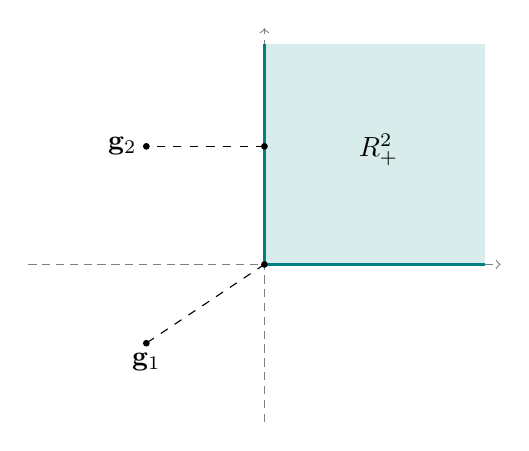
\begin{tikzpicture}
            \draw[densely dashed, gray][->] (0, -2) -- (0, 3);
            \draw[densely dashed, gray][->] (-3, 0) -- (3, 0);
            \path[fill=teal, fill opacity = 0.15] (0, 0) -- (0, 2.8) -- (2.8, 2.8) -- (2.8, 0) -- (0, 0) -- cycle;
            \draw[teal, line width=1pt] (0, 0) -- (0, 2.8);
            \draw[teal, line width=1pt] (0, 0) -- (2.8, 0);
            \filldraw (0, 0) circle (1pt);

            \begin{scope}
                \filldraw (-1.5, -1) circle (1pt);
                \draw[dashed] (0, 0) -- (-1.5, -1);
                \node at (-1.5, -1) [below]{$\mathbf{g}_1$};
            \end{scope}
            \begin{scope}
                \filldraw (-1.5, 1.5) circle (1pt);
                \filldraw (0, 1.5) circle (1pt);
                \draw[dashed] (0, 1.5) -- (-1.5, 1.5);
                \node at (-1.5, 1.5) [left]{$\mathbf{g}_2$};
            \end{scope}
            \node at (1.45, 1.45) {$\mathbb{R}^2_+$};
        \end{tikzpicture}
        \caption{}
    \end{subfigure}
    \caption{\centering Examples of cones used for computation of statistical dimension in examples~\ref{ex:1}~and~\ref{ex:2}}
    \label{fig:cones}
\end{figure}

\begin{example}\label{ex:1}
    Let $\mathcal{C} \subset \mathbb{R}^2 $ be a convex cone as shown in Fig.~\ref{fig:cones_a}.
    It has one zero-dimensional face (\{$\mathbf{0}$\}, the origin point), two one-dimensional faces (the two boundary rays)
    and one two-dimensional face (the cone itself).
    For the projection of vector $\mathbf{g}$ to be in the relative interior of a zero-dimensional face (which is also $\{\mathbf{0}\}$),
    the vector $\mathbf{g}$ has to be inside of the polar of $\mathcal{C}$, i.e., $\mathbf{g} \in \mathcal{C}^*$.
    The standard normal distribution is rotationally symmetric, so $\mathbb{P}\{ \mathbf{g} \in \mathcal{C}^*\} = \frac{\pi - \phi}{2\pi} $.
    Similarly, for $\op{proj}_{\mathca{C}} \mathbf{g}$ to lie inside $\mathcal{C}$, $\mathbf{g}$ itself must be inside of $\mathcal{C}$,
    which happens with probability $\frac{\phi}{2\pi}$.
    Finally, for one-dimensional faces we have the probability $\frac{1}{2}$.
    The statistical dimension can be easily calculated from the definition as
    \[ \delta (\mathcal{C}) = \frac{1}{2} + 2\frac{\phi}{2\pi} = \frac{\pi + 2\phi}{2\pi}.\]
\end{example}

\begin{example}\label{ex:2}
    The non-negative orthant $\mathbb{R}^N_+$ forms a polyhedral cone as an intersection of two half-spaces.
    It has one zero-dimensional face $\{\mathbf{0}\}$, $N$ one-dimensional faces of the form $\{0\}^k \times \mathbb{R}_+ \times \{0\}^{N-k-1}$
    for $k \in [\![ 0..N-1 ]\!]$, $\frac{N(N-1)}{2}$ two-dimensional faces of the form
    $\{0\}^k \times \mathbb{R}_+ \times \{0\}^j \times \mathbb{R}_+ \times \{0\}^{N-k-j-2}$ for
    $(k, j) \in  [\![ 0..N-2 ]\!]^2$ with $k+j = N-2$ and so on.
    In other words, $k$-dimensional faces only contain vectors with exactly $k$ non-zero components.
    Then $\op{proj}_{\mathbb{R}^N_+} \mathbf{g}$ lies in the relative interior of a $k$-dimensional face of $\mathbb{R}^N_+$
    if and only if $\mathbf{g}$ has exactly $k$ positive components, so
    \begin{equation*}
        {\nu_k(\mathbb{R}^N_+) = \mathbb{P}\{ \mathbf{g} \text{ has exactly } k \text{ positive components} \} }.
    \end{equation*}
    There are $\binom{N}{k}$ ways to ``choose'' which components will be positive.
    The probability of each component to be positive is $1/2$; the probability of it to be negative is also $1/2$.
    As they are independent from each other, we get the result
    \[{\nu_k(\mathbb{R}^N_+) = \frac{1}{2^N} \binom{N}{k}. \]
    The statistical dimension is then
    \[\delta (\mathbb{R}^N_+) = \frac{1}{2^N}\sum_{k=0}^N k \binom{N}{k} = \frac{N}{2^N} \sum_{k=0}^{N-1} \binom{N-1}{k} = \frac{N}{2}.\]
    For example, $\delta(\mathbb{R}_+) = 1/2$ and $\delta(\mathbb{R}_+^2)=1$.
\end{example}

\begin{figure}
    \begin{subfigure}{0.5\textwidth}
            \includegraphics[width=\linewidth]{pictures/lote_estimates}
        \caption{}
    \end{subfigure}
    \begin{subfigure}{0.5\textwidth}
            \includegraphics[width=\linewidth]{pictures/lote_estimates_d300}
        \caption{}
    \end{subfigure}

    \caption{\centering Results of numerical experiments in dimensions 100 and 300. Yellow line corresponds to the estimated statistical
    dimension of the descent cone.}
    \label{fig:lote}
\end{figure}

The topic of statistical dimension and conic intrinsic volumes is discussed in more detail in~\cite{statdim}.
Now we can look at the main result of this paper that predicts the location of the phase transition, as well as gives
minimal number of measurements corresponding to a desired level of success.
\begin{theorem}
    Let $\x^* \in \mathbb{R}^N$ be a fixed vector and $p \in (0, 1)$.
    Suppose $\A \in M_{m \times N}(\mathbb{R})$ is a matrix with independent $\mathcal{N}(0,1)$-distributed entries and
    $\y = \A \x^*$.
    Then
    \begin{align*}
        & m \leq \delta(\mathcal{D}(\norm{\cdot}_1, \x^*)) - a_\eta \sqrt{N} \implies
        \mathbb{P}\{\x^* \text{ is the unique solution of \ref{eq:l1}}\} \leq \eta
        \\
        & m \geq \delta(\mathcal{D}(\norm{\cdot}_1, \x^*)) + a_\eta \sqrt{N} \implies
        \mathbb{P}\{\x^* \text{ is the unique solution of \ref{eq:l1}}\} \geq 1 - \eta,
    \end{align*}
    where $a_\eta = \sqrt{8 \log (4/\eta)}$.
    \label{th:lote}
\end{theorem}

Fig.~\ref{fig:lote} shows the estimates from this theorem and the statistical dimension plotted over
the results of numerical experiments.
We can see that the curve of statistical dimension sits exactly in the middle of the transition region;
we also observe both the bounds and the transition region becoming relatively thinner in higher dimension.

\begin{remark}
    In the paper, authors only show on plots the curve corresponding to the statistical dimension and omit the actual estimates for $m$,
    which are plotted in blue and red here.
    And understandably so --- those predictions look terrible in dimension 100; at first I thought I had made a mistake in the code, as
    they look even worse than the ones given by the previous paper (\cite{convexgeom}), that was published a year earlier.
    However, we also see that situation gets better in bigger dimension; moreover, from the statement of the theorem itself we can
    predict that the relative width of the region between these two lines will approach 0 as $N \to \infty$.
    We can observe that behavior in Fig.~\ref{fig:compare}, where we also plot the curve for $m$ from \ref{th:log_improved}.
    To try and make this comparison fair, we fix the same probability (0.95) for both results, based on the probability
    estimate in \ref{th:log_improved}.
    Though we have to keep in mind that this estimate is less optimistic than the original statement of \ref{th:log},
    so this comparison might still be a bit unfair.
\end{remark}

\begin{figure}
    \begin{subfigure}{0.5\textwidth}
        \includegraphics[width=\linewidth]{pictures/compare_estimates1000}
    \end{subfigure}
    \begin{subfigure}{0.5\textwidth}
        \includegraphics[width=\linewidth]{pictures/compare_estimates10000}
    \end{subfigure}
    \caption{\centering Comparison of different estimates in higher dimensions.}
    \label{fig:compare}
\end{figure}